% ===========================================================================
\section{Results}
\label{sec:results}
% ===========================================================================

\subsection{National greenhouse-gas inventory}

Pakistan's agricultural emissions in 2024 are estimated at \SI{223.5}{}~Mt~\COe{} using AR5
GWP-100 values. The corresponding AR6 total is \SI{218.1}{}~Mt~\COe{}.

Enteric fermentation is the largest category, contributing \SI{151.7}{}~Mt~\COe{}, or
\SI{68}{\percent} of the national agricultural total. Managed soils contribute
\SI{28.5}{}~Mt~\COe{}, followed by manure management at \SI{21.2}{}~Mt~\COe{} and rice
cultivation at \SI{16.5}{}~Mt~\COe{}. Urea application contributes \SI{4.8}{}~Mt~\COe{},
while field burning of crop residues contributes \SI{0.7}{}~Mt~\COe{}.

The inventory is therefore dominated by livestock. Enteric fermentation and manure management
together account for approximately \SI{78}{\percent} of the total. Soil and rice emissions
make up most of the remainder.

\begin{table}[!htbp]
\centering
\footnotesize
\begin{tabular}{@{}lccc@{}}
\toprule
\textbf{Category (IPCC code)} & \textbf{AR5} & \textbf{AR6} & \textbf{$\pm$\%} \\
\midrule
Enteric fermentation (3.A)   & 151.7 & 146.2 & 25 \\
Manure management (3.B)      &  21.2 &  21.0 & 33 \\
Managed soils (3.D)          &  28.5 &  29.4 & 47 \\
Rice cultivation (3.C)       &  16.5 &  16.0 & 61 \\
Urea application (3.H)       &   4.8 &   4.8 & 11 \\
Field burning (3.F)          &   0.7 &   0.7 & 45 \\
\midrule
\textbf{Agriculture total}   & \textbf{223.5} & \textbf{218.1} & \textbf{19} \\
\bottomrule
\end{tabular}
\caption{Agricultural greenhouse-gas emissions by IPCC category, 2024, reported in
Mt~\COe{} using AR5 and AR6 GWP-100 values. The uncertainty column reports the IPCC
Approach~1 \SI{95}{\percent} relative half-width.}
\label{tab:national}
\end{table}

\subsection{Comparison with international inventories}

The category-level comparison with FAOSTAT uses 2023, the latest common year, and includes
only the five agricultural categories reported by both inventories. Urea and liming are
excluded from this comparison because FAOSTAT does not report corresponding lines for
Pakistan.

The engine values compared are the calendar-2023 reconstruction of the fiscal series
(Table~\ref{tab:benchmark}), not the FY2023--24 totals reported above, which sit on a
different twelve months. For these five categories, our estimate is
\SI{207.8}{}~Mt~\COe{}, compared with \SI{233.3}{}~Mt~\COe{} in FAOSTAT. The resulting
ratio is \num{0.89}.

Agreement differs among categories. Enteric fermentation agrees to within five per cent, with a
ratio of \num{0.99}. Rice cultivation and field burning have ratios of \num{1.16} and
\num{0.91} respectively. Manure-management emissions are \num{1.38} times the FAOSTAT value.

Managed soils show the largest difference. Our estimate is \SI{27.1}{}~Mt~\COe{}, compared
with \SI{58.5}{}~Mt~\COe{} in FAOSTAT, giving a ratio of \num{0.46}. As discussed in
Section~\ref{sec:discussion}, this difference is driven mainly by the selected direct-soil
emission factor: the present inventory uses the 2019 dry-climate factor of $0.005$, whereas
FAOSTAT retains the older aggregate value of $0.010$.

The 1990--2023 reconstruction uses FAOSTAT activity series. The comparison with FAOSTAT
therefore primarily evaluates the implementation and the consequences of different emission
factors. The close reproduction of the FAOSTAT enteric series indicates that the livestock
calculation has been implemented consistently, but it does not independently confirm the
underlying activity data.

Full-scope comparisons include urea application and use the GWP basis reported by each
benchmark. The inventory is \num{0.80} times the EDGAR estimate in 2023 and \num{0.86} times
EDGAR in 2024. Climate TRACE reports AR6 values; on that basis, our 2024 total is \num{0.83}
times the Climate TRACE estimate. The higher EDGAR and Climate TRACE totals arise mainly from
their larger estimates of enteric methane.

\begin{table}[!htbp]
\centering
\footnotesize
\begin{tabular}{@{}lccc@{}}
\toprule
\textbf{Category (2023, AR5)} & \textbf{Engine} & \textbf{FAOSTAT} & \textbf{Ratio} \\
\midrule
Enteric fermentation & 143.2 & 145.1 & 0.99 \\
Manure management    &  20.2 &  14.6 & 1.38 \\
Rice cultivation     &  16.5 &  14.3 & 1.16 \\
Managed soils        &  27.1 &  58.5 & 0.46 \\
Field burning        &   0.7 &   0.8 & 0.91 \\
\midrule
\textbf{Agriculture subtotal (ex urea/lime)} & \textbf{207.8} & \textbf{233.3} & \textbf{0.89} \\
\midrule
\multicolumn{4}{@{}l}{\emph{Full-scope totals (engine incl.\ urea) vs urea-inclusive inventories}} \\
vs EDGAR 2023 (AR5)  & 212.6 & 267.4 & 0.80 \\
vs EDGAR 2024 (AR5)  & 223.5 & 261.2 & 0.86 \\
vs Climate TRACE 2024 (AR6)$^{a}$ & 218.1 & 261.5 & 0.83 \\
\bottomrule
\end{tabular}
\caption{Comparison with international agricultural inventories using matched
years, category scope and GWP basis. Category-level rows compare the five categories reported
by both this inventory and FAOSTAT in 2023. Full-scope rows compare the inventory, including
urea application, with EDGAR and Climate TRACE; the EDGAR 2023 row is from the prior
2024-vintage booklet \citep{edgar2024} and the EDGAR 2024 row from the 2025 release
\citep{edgar2025booklet}, retained together because the 2025 release revised the
agricultural \CHfour{} history. Climate TRACE is compared using AR6 values.}
\label{tab:benchmark}
\end{table}

\subsection{Effect of stream-specific spatial allocation}
\label{sec:results-proxies}

Broad inventory categories are not spatially homogeneous. Managed soils provide the clearest
example, because the category includes nitrogen from synthetic fertiliser, applied manure,
pasture deposition and crop residues. Approximately three-fifths of the nitrogen in this
category is livestock-derived.

Allocating all managed-soils emissions with one fertiliser or cropland proxy would therefore
misrepresent much of the category. The framework allocates each nitrogen stream separately
using the proxy associated with the process that generates it, and the stream-level surfaces
are then summed to produce the category map.

Three allocation changes affect the provincial geography.

First, indirect \NtwoO{} from volatilisation and leaching was divided by nitrogen source.
Previously each pathway was allocated as one aggregate stream using fertiliser offtake, even
though synthetic fertiliser accounts for only approximately \SI{30}{\percent} of volatilised
nitrogen and \SI{37}{\percent} of leached nitrogen. Allocating the synthetic, manure, residue
and pasture components separately shifts \SI{2.28}{}~Mt~\COe{} out of Punjab.

Second, applied manure was moved from livestock density alone to the cell-level intersection
of cropland and livestock density. Livestock density represents where manure is produced,
whereas cropland represents where it can be applied; their intersection identifies cultivated
areas located close to livestock production. This change shifts \SI{2.08}{}~Mt~\COe{} back to
Punjab.

The intersection surface is not a simple average of its two components. In Sindh, livestock
and cropland are concentrated in the same Indus corridor, so the intersection produces a
larger provincial share than either parent proxy alone. In Balochistan, much of the livestock
population occupies rangelands with little nearby cropland, so the intersection produces a
smaller share than either parent proxy.

Third, synthetic nitrogen applied to rice was moved from provincial fertiliser offtake to
mapped paddy area. This produces only a small provincial change.

These revisions redistribute emissions within the fixed national and provincial control
system. They do not change the national magnitude. Their combined net provincial effect is
small because the first two changes largely offset, but each produces a substantial
redistribution when considered separately.

Splitting physical streams also affects uncertainty propagation. Components derived from the
same physical flux may use different spatial proxies while retaining a shared emission
factor. Treating the components as statistically independent would reduce the uncertainty
merely because the stream had been divided into more rows. The analytical calculation
therefore combines components sharing $EF_4$ or $EF_5$ linearly before applying the
quadrature step, and the Monte-Carlo calculation uses one shared deviate for each correlated
group. Managed-soils uncertainty remains $\pm$47\% under this treatment.

\begin{table}[!htbp]
\centering
\footnotesize
\setlength{\tabcolsep}{4pt}
\begin{tabular}{@{}lrrrr@{}}
\toprule
& \multicolumn{3}{c}{\textbf{Change}} & \\
\cmidrule(lr){2-4}
\textbf{Province} & \textbf{Split indirect} & \textbf{Manure proxy} & \textbf{Rice proxy}
& \textbf{Net} \\
\midrule
Punjab             & $-2.28$ & $+2.08$ & $+0.04$ & $-0.17$ \\
Sindh              & $-0.33$ & $+0.50$ & $-0.03$ & $+0.14$ \\
Khyber Pakhtunkhwa & $+1.17$ & $-1.22$ & $-0.02$ & $-0.08$ \\
Balochistan        & $+1.45$ & $-1.35$ & $+0.01$ & $+0.11$ \\
\bottomrule
\end{tabular}
\caption{Changes in provincial allocation produced by separating indirect
\NtwoO{} by nitrogen source, replacing the applied-manure proxy, and assigning rice-specific
fertiliser to mapped paddy area. Values are reallocations in Mt~\COe{} and sum to zero
nationally. The small net effect results from offsetting shifts and does not imply that the
individual changes are unimportant.
Generated by
\texttt{src/pkinv/eval/proxy\_attribution.py}.}
\label{tab:proxyattr}
\end{table}

\subsection{Provincial and gridded distribution}

Agricultural emissions are concentrated in the irrigated Indus basin.

Punjab contributes \SI{123.3}{}~Mt~\COe{}, or \SI{55}{\percent} of the national total. Sindh
contributes \SI{51.4}{}~Mt~\COe{}, or \SI{23}{\percent}. Khyber Pakhtunkhwa contributes
\SI{31.0}{}~Mt~\COe{}, or \SI{14}{\percent}, and Balochistan contributes
\SI{17.3}{}~Mt~\COe{}, or \SI{8}{\percent}. A small residual of approximately
\SI{0.4}{}~Mt~\COe{} occurs outside the four provincial totals.

The \SI{0.05}{\degree} total-emissions surface follows the canal-irrigated agricultural
corridor. Emissions decline sharply across arid western Balochistan and the northern mountain
regions.

The category maps have distinct spatial patterns because they use different process-specific
proxies. Enteric fermentation and manure management extend into livestock-producing
rangelands and settlements. Rice methane follows mapped paddy area. Crop-residue burning is
concentrated in the Punjab rice--wheat belt, where satellite fire detections are most
frequent.

\begin{table*}[!htbp]
\centering
\footnotesize
\begin{tabular}{@{}lcccccc@{}}
\toprule
\textbf{Province} & \textbf{Ent.} & \textbf{Man.} & \textbf{Rice}
& \textbf{Soils} & \textbf{Urea} & \textbf{Total} \\
\midrule
Punjab             & 79.9 & 10.3 & 12.2 & 17.1 & 3.3 & 123.3 \\
Sindh              & 35.8 &  4.7 &  3.4 &  6.4 & 1.1 &  51.4 \\
Khyber Pakhtunkhwa & 24.3 &  3.7 &  0.3 &  2.5 & 0.2 &  31.0 \\
Balochistan        & 11.4 &  2.5 &  0.7 &  2.6 & 0.1 &  17.3 \\
Other              &  0.3 &  0.0 &  0.0 &  0.0 & 0.0 &   0.4 \\
\midrule
\textbf{National}  & \textbf{151.7} & \textbf{21.2} & \textbf{16.5}
& \textbf{28.5} & \textbf{4.8} & \textbf{223.5} \\
\bottomrule
\end{tabular}
\caption{Provincial greenhouse-gas emissions by category in 2024, reported in
Mt~\COe{} using AR5 GWP-100. Field burning is included in the total but omitted as a separate
column for space. Provincial rows reproduce the national category totals exactly.}
\label{tab:provincial}
\end{table*}

\begin{figure}[!htbp]
\centering
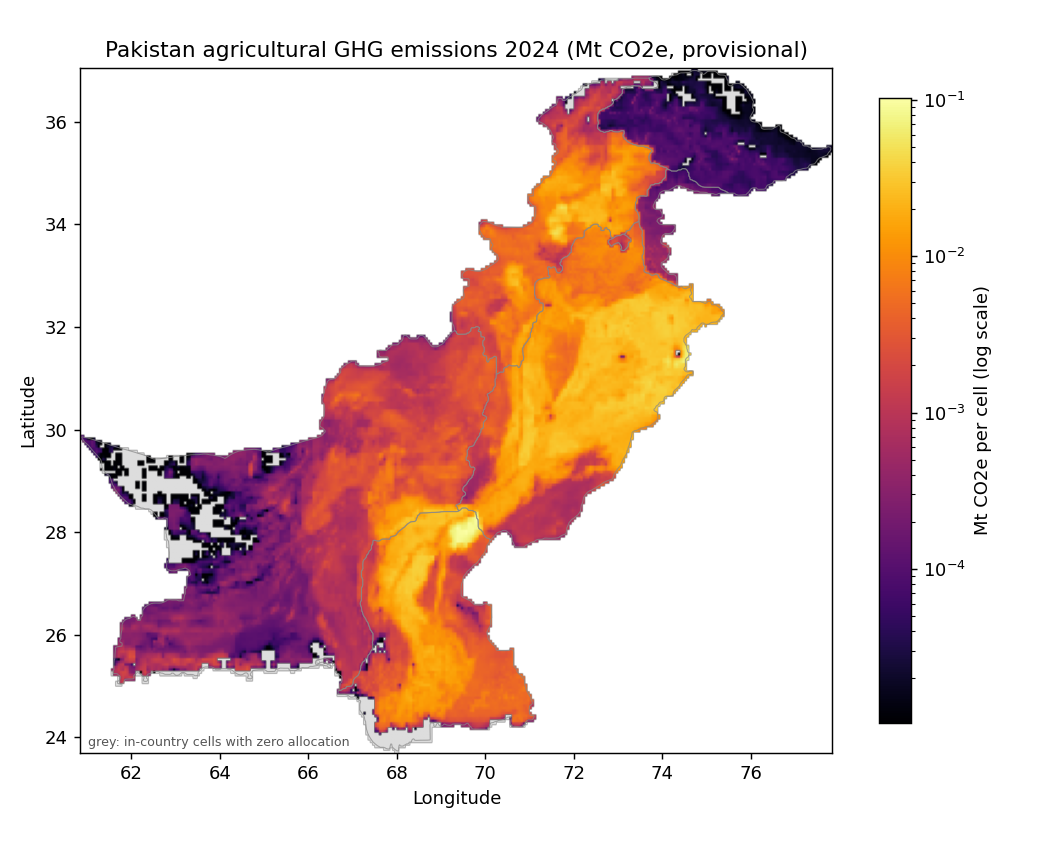
\includegraphics[width=\linewidth]{hotspot_total.png}
\caption{Total agricultural greenhouse-gas emissions on the \SI{0.05}{\degree}
grid in 2024, reported as Mt~\COe{} per cell on a logarithmic scale. The gridded surface
reproduces the provincial and national control totals.}
\label{fig:hotspot}
\end{figure}

\begin{figure*}[!htbp]
\centering
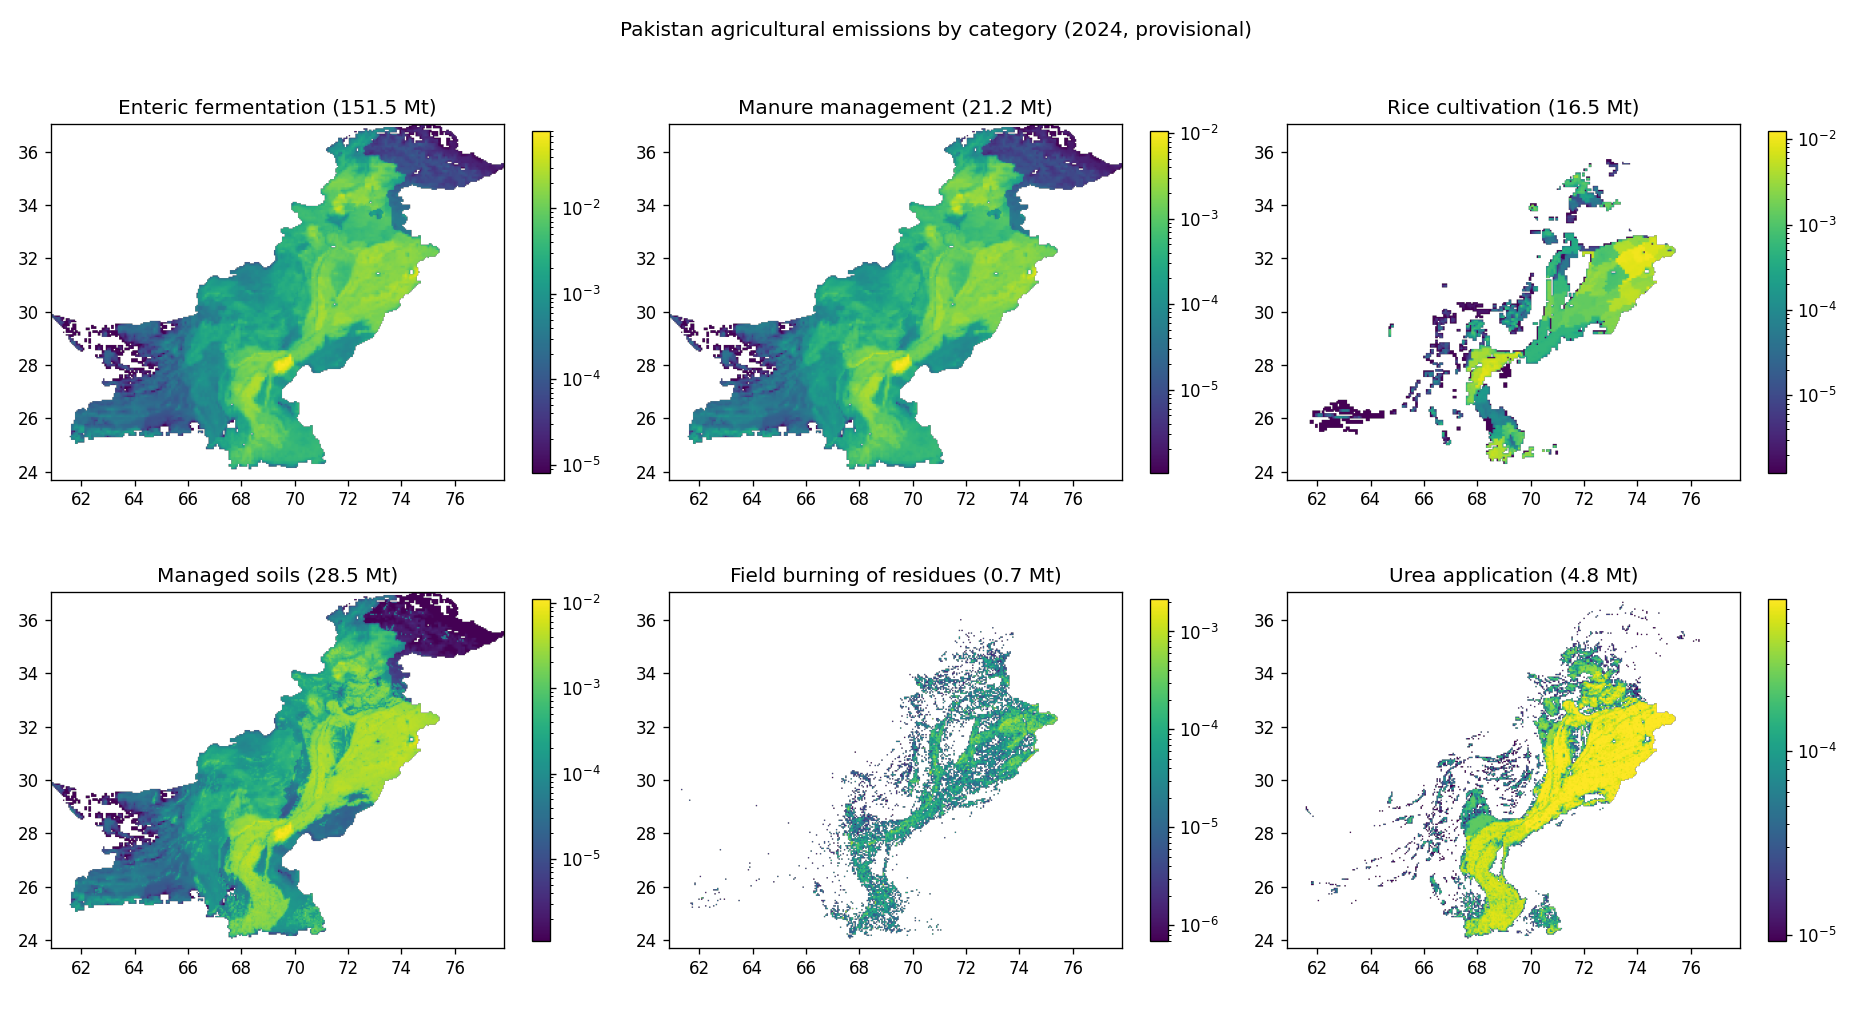
\includegraphics[width=\textwidth]{hotspot_by_category.png}
\caption{Agricultural emissions by category. Livestock emissions follow
species-weighted livestock density, rice methane follows mapped paddy area, and crop-residue
burning follows satellite fire occurrence. Each panel uses its own logarithmic scale; colours
should not be compared directly between categories.}
\label{fig:bycat}
\end{figure*}

\begin{figure}[!htbp]
\centering
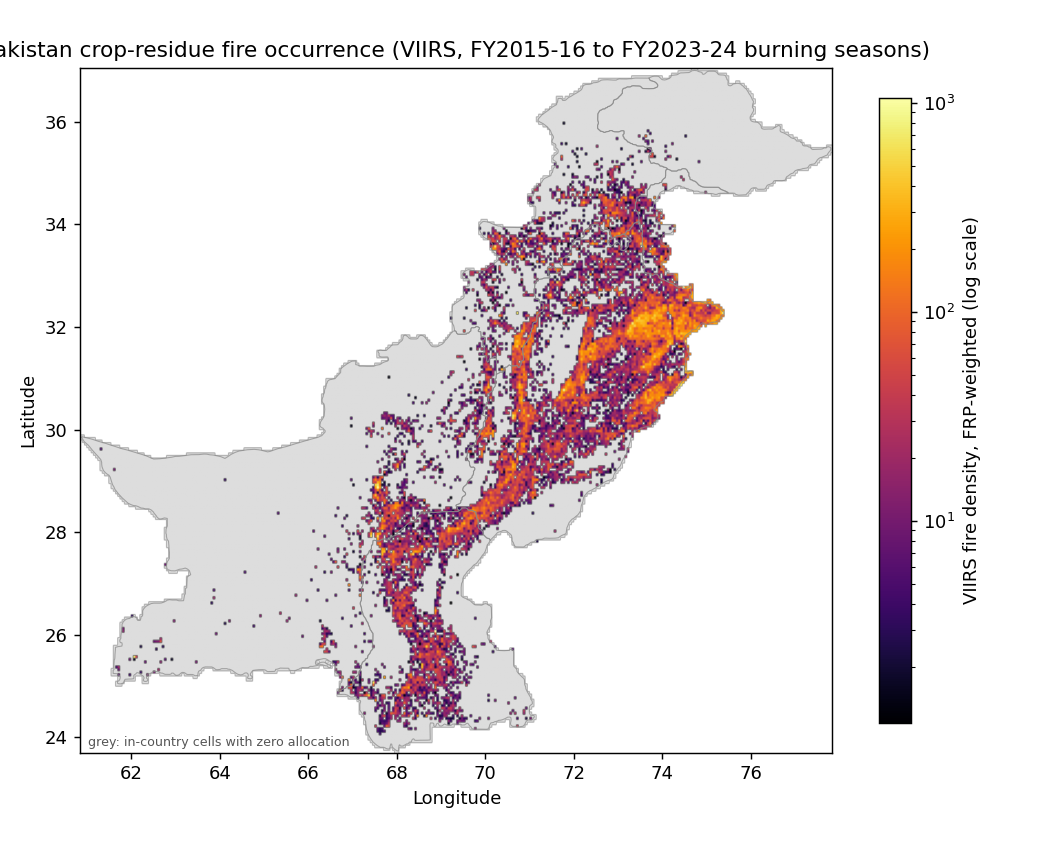
\includegraphics[width=\linewidth]{fire_occurrence.png}
\caption{NASA FIRMS VIIRS active-fire detections used to allocate crop-residue
burning, from the FY2023--24 reporting period's own season: post-monsoon rice-stubble
burning (October--December 2023) and spring wheat-residue burning (April--May 2024),
concentrated mainly in Punjab's rice--wheat belt.}
\label{fig:fire}
\end{figure}

\subsection{District distribution}
\label{sec:results-district}

District allocation resolves the provincial totals to 116 districts and one residual
reporting unit (114 with a boundary polygon, and the two census units---Cholistan Area
and Larkana District---that the boundary file does not draw, carried as named rows on the
province surface)---the four-province base that matches the provincial scope of the
activity statistics, narrower by design than the 134-district census frame the
residential and waste sectors allocate over. This scale corresponds more closely to the
administrative level at which
agricultural and air-quality interventions are commonly implemented.

Most of the highest-emitting districts are located in the central and southern Punjab canal
belt, with one exception at the head of the table. Karachi has the largest estimated total at
\SI{10.18}{}~Mt~\COe{}: the 2024 census enumerates the division's seven districts
separately---\SI{2.8}{} million cattle and \SI{3.6}{} million buffalo, Malir's peri-urban
dairy colonies the largest part---and all seven resolve onto the one Karachi polygon through
the canonical district crosswalk, where earlier releases had placed the shape on the GLW
surface (\SI{0.10}{}~Mt) because none of the seven census names matched it. Jhang follows
at \SI{8.61}{}~Mt~\COe{} and Sheikhupura at \SI{6.73}{}~Mt~\COe{}. Faisalabad and
Muzaffargarh contribute \SI{6.3}{} and \SI{5.8}{}~Mt~\COe{}. The rice-belt
concentration sharpened in this release: rice cultivation now rides the MapSPAM
surface rather than the generic cropland fallback, which lifts the classic
rice districts (Sheikhupura, and Sialkot and Kasur into the table) and is scored
against the Punjab Crop Reporting Service in the spatial benchmarks.

These districts rank highly because they combine large livestock populations, intensively
fertilised cropland and, in some cases, rice production.

Two limits of the district layer are published rather than described, and since rc41 each is
priced as the fraction of every affected stream's own mass that rode the substitute surface,
at that stream's gas and methane origin---earlier releases quoted the whole module mass of the
affected unit, summed across gases without a warming potential. One census unit, Larkana
District, has no polygon of its own in the boundary file, so a stream whose district panel
places mass in it falls back to a within-province spread: the provincial total is unaffected
and the sub-provincial placement of \SI{2.56}{}~Mt~\COe{} across the agriculture,
residential and waste streams is not made. The same class
carries the panel mass of the territories outside the four provinces (ICT, GB, AJK), for which
the district frame has no shapes: \SI{0.35}{}~Mt~\COe{} across agriculture and residential.
In seven shapes the MapSPAM surface shows no paddy at all, so the rice-specific fertiliser
stream is spread uniformly inside them rather than by the declared surface, affecting
\SI{0.029}{}~Mt~\COe{}. All three are listed with their masses and whether they are resolvable in
\texttt{outputs/pakemis\_spatial\_exceptions.csv}. Summing the district layer back over each
province reproduces the provincial allocation exactly
(\texttt{outputs/pakemis\_adm2\_nesting\_check.csv}): each shape's mass is partitioned
among the reporting units of its own province only, so no mass crosses a provincial boundary
between the allocation and the district table.

Matiari in Sindh is the other entry from outside Punjab. Its estimated total
is \SI{4.28}{}~Mt~\COe{} (ninth). Unlike the leading Punjab districts, its total is driven mainly
by livestock density rather than extensive crop cultivation. The category-level
decomposition makes this difference visible.

\begin{table}[!htbp]
\centering
\footnotesize
\begin{tabular}{@{}rllc@{}}
\toprule
\textbf{\#} & \textbf{District} & \textbf{Province} & \textbf{Mt~\COe} \\
\midrule
1  & Karachi           & Sindh  & 10.18 \\
2  & Jhang             & Punjab & 8.61 \\
3  & Sheikhupura       & Punjab & 6.73 \\
4  & Faisalabad        & Punjab & 6.32 \\
5  & Muzaffargarh      & Punjab & 5.84 \\
6  & Dera Ghazi Khan   & Punjab & 4.96 \\
7  & Bahawalnagar      & Punjab & 4.47 \\
8  & Sargodha          & Punjab & 4.43 \\
9  & Matiari           & Sindh  & 4.28 \\
10 & Rahim Yar Khan    & Punjab & 4.14 \\
11 & Okara             & Punjab & 3.98 \\
12 & Bahawalpur        & Punjab & 3.81 \\
13 & Sialkot           & Punjab & 3.74 \\
14 & Kasur             & Punjab & 3.72 \\
15 & Gujranwala        & Punjab & 3.65 \\
\bottomrule
\end{tabular}
\caption{Fifteen districts with the highest total agricultural
greenhouse-gas emissions in 2024, reported in Mt~\COe{} using AR5 GWP-100. District estimates
sum to the provincial and national control totals.}
\label{tab:districttop}
\end{table}

\begin{figure}[!htbp]
\centering
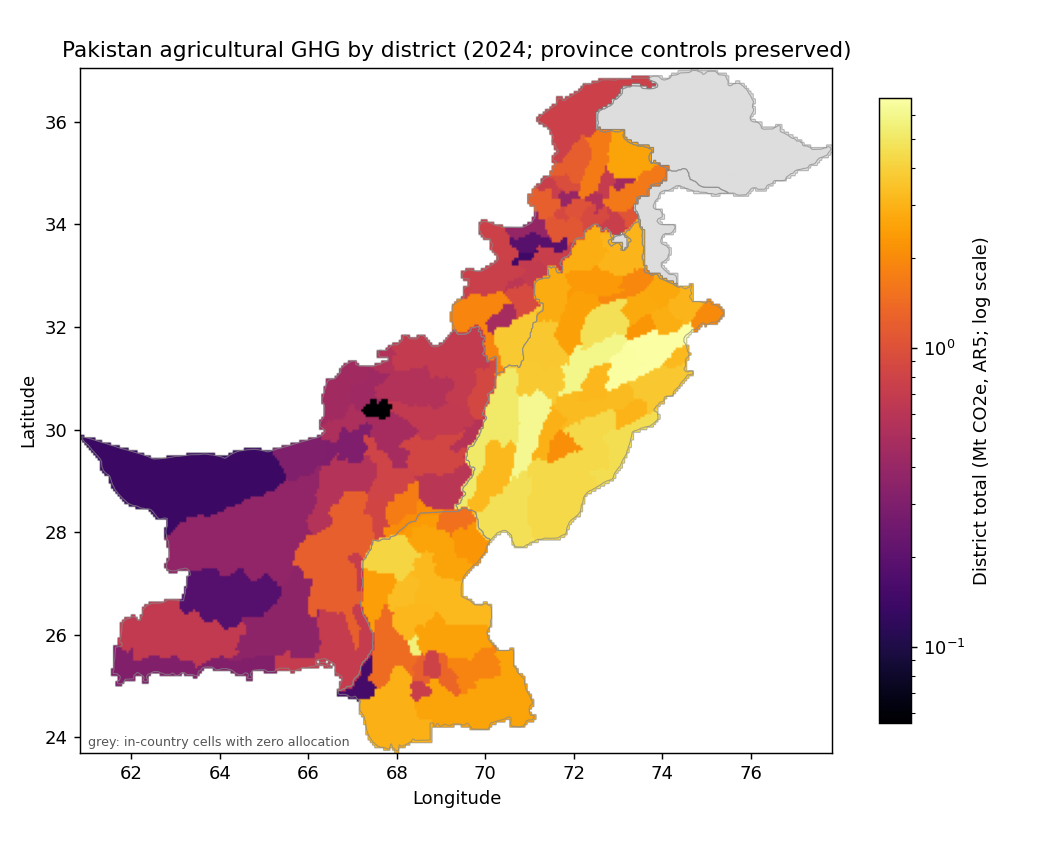
\includegraphics[width=\linewidth]{district_totals.png}
\caption{Agricultural greenhouse-gas emissions by district in 2024. Values
are shown as annual emissions per unit area, allowing districts of different sizes to be
compared. The underlying district totals reproduce the provincial and national inventory.}
\label{fig:districtmap}
\end{figure}

\subsection{National trajectory, 1990--2024}

Agricultural greenhouse-gas emissions increase from approximately \SI{83}{}~Mt~\COe{} in 1990
to \SI{223.5}{}~Mt~\COe{} in 2024. This corresponds to a compound annual growth rate of
approximately \SI{2.9}{\percent}.

The increase is driven mainly by growth in livestock populations and synthetic-fertiliser
use. Emission factors are held constant throughout the series, so the trajectory represents
changes in reported activity rather than changes in methodological assumptions.

The 1990--2023 series uses FAOSTAT activity data on a \emph{calendar-year} basis;
the 2024 value is anchored to the PBS agricultural census and other current
Pakistani sources on the \emph{FY2023--24 fiscal} basis. The join is therefore a
time-basis break as well as a source break---the last FAOSTAT point covers
January--December 2023 while the anchor covers July 2023--June 2024, an overlap of
six months---and the published series carries a \texttt{year\_basis} column
(\texttt{calendar\_faostat} / \texttt{fiscal\_census\_anchor}) so no reader can
treat the two segments as one homogeneous fiscal series. Part of the change between
2023 and 2024 may reflect either transition. This issue is discussed in
Section~\ref{sec:limitations}.

\begin{figure}[!htbp]
\centering
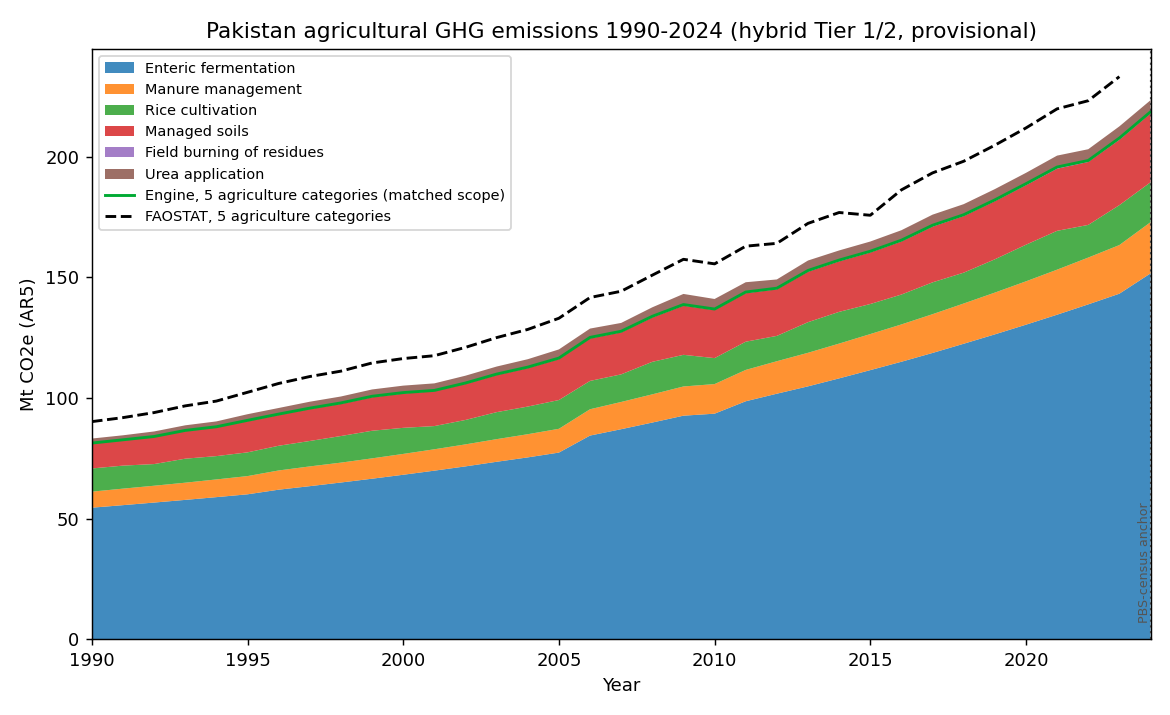
\includegraphics[width=\linewidth]{trend_chart.png}
\caption{Agricultural greenhouse-gas emissions by category, 1990--2024. The
benchmark lines compare this inventory with FAOSTAT using the five categories reported by both
systems. The vertical marker identifies the 2024 transition from the calendar-year FAOSTAT
activity series to the fiscal-year PBS census anchor---a time-basis break as well as
a source break, flagged per row in the published series.}
\label{fig:trend}
\end{figure}

\subsection{Historical district panel}
\label{sec:results-districtyear}

Applying the fixed 2024 district shares to the national time series produces a
district-by-category panel for 1990--2024. The panel contains \num{24290}
district-year-category records and reconciles to the national inventory in every year.

Under the fixed-share assumption, district trajectories follow the national trend.
Sheikhupura increases from approximately \SI{2.9}{}~Mt~\COe{} in 1990 to
\SI{6.7}{}~Mt~\COe{} in 2024. Faisalabad increases from \SI{2.4}{} to \SI{6.6}{}~Mt~\COe{},
and Muzaffargarh from \SI{2.4}{} to \SI{5.8}{}~Mt~\COe{}.

These trajectories should be interpreted as a spatial distribution of the national historical
series. They do not show observed district-specific changes in livestock, cropping patterns
or fertiliser use. Measuring such changes would require consistent historical activity data
at district level. The panel now carries that qualification per row rather than only here:
every record outside the reference year is marked \texttt{reference\_shape\_backcast}, and
only the \num{694} reference-year records are the audited district pattern. A reader who
opens the CSV without this section still cannot mistake a 1990 row for a 1990 observation.

Despite this limitation, the panel provides a district-resolved historical baseline that
remains numerically consistent with the national inventory.

\begin{figure}[!htbp]
\centering
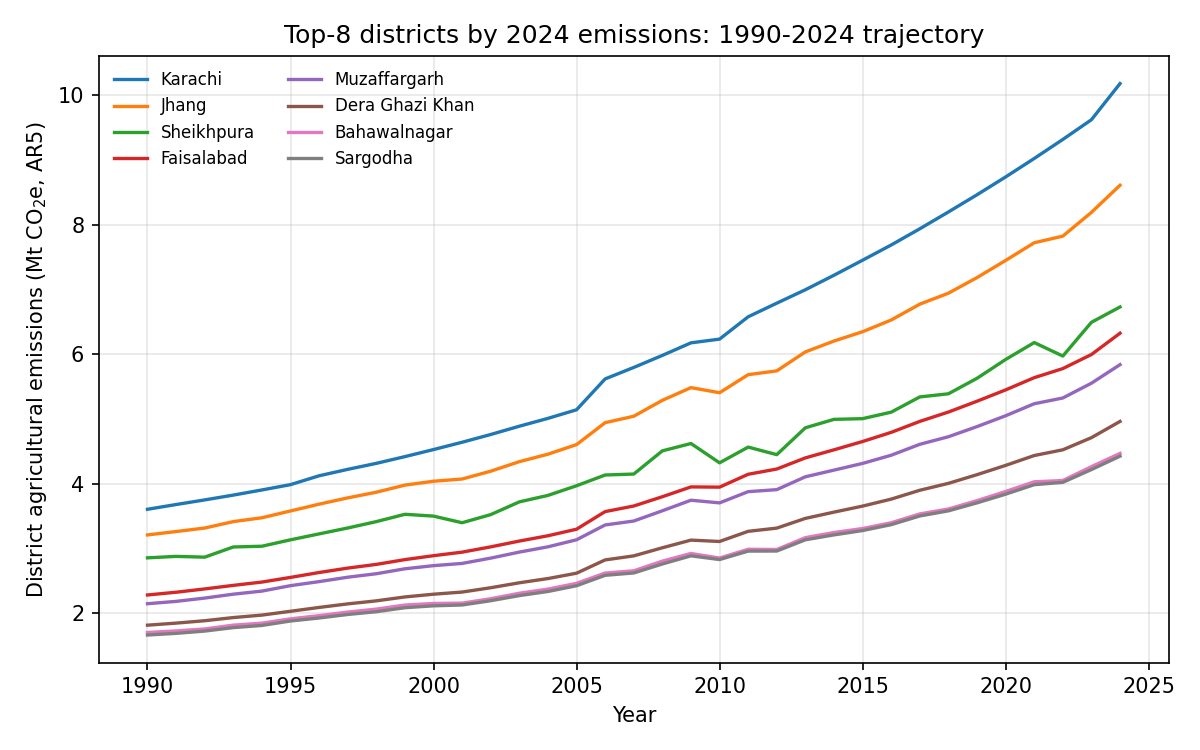
\includegraphics[width=\linewidth]{district_trajectory.png}
\caption{Agricultural greenhouse-gas trajectories for the eight
highest-emitting districts, 1990--2024. District values use fixed 2024 spatial shares and
reproduce the national control total in every year.}
\label{fig:districttraj}
\end{figure}

\subsection{Parametric uncertainty}

The IPCC Approach~1 calculation gives a \SI{95}{\percent} relative half-width of $\pm$19\%
for the national agricultural total.

The Monte-Carlo analysis produces a mean of \SI{223.7}{}~Mt~\COe{}, close to the
deterministic estimate of \SI{223.5}{}~Mt~\COe{}. Its median is \SI{222.3}{}~Mt~\COe{}, and
its \SI{95}{\percent} interval is \SI{185.3}{}--\SI{270.9}{}~Mt~\COe{}. This corresponds to a
relative half-width of approximately \SI{19.2}{\percent}.

The close agreement indicates that the national interval is not highly sensitive to whether
the documented uncertainties are propagated analytically or through mean-preserving lognormal
sampling. Both calculations use the same underlying assumptions and the correlation treatment
described in Section~\ref{sec:methods}.

Rice cultivation has the widest category-level uncertainty at $\pm$62\%, reflecting
uncertainty in cultivation conditions and the assumed water regime. Managed soils follow at
$\pm$47\%, largely because of uncertainty in direct and indirect \NtwoO{} factors. Urea
application has the narrowest interval at $\pm$11\%.

These results show that improved information on rice water management and soil \NtwoO{}
factors would reduce national inventory uncertainty more than further refinement of the urea
calculation.

\begin{table*}[!htbp]
\centering
\footnotesize
\begin{tabular}{@{}lccccc@{}}
\toprule
\textbf{Category} & \textbf{Mean} & \textbf{P2.5} & \textbf{P50} & \textbf{P97.5}
& \textbf{$\pm$\%} \\
\midrule
Enteric fermentation & 151.9 & 117.9 & 150.7 & 194.3 & 25 \\
Manure management    &  21.2 &  15.8 &  20.7 &  29.8 & 33 \\
Managed soils        &  28.5 &  17.9 &  27.5 &  44.5 & 47 \\
Rice cultivation     &  16.6 &   8.7 &  15.8 &  28.6 & 61 \\
Urea application     &   4.8 &   4.3 &   4.8 &   5.4 & 11 \\
Field burning        &   0.7 &   0.4 &   0.7 &   1.0 & 45 \\
\midrule
\textbf{Total}       & \textbf{223.7} & \textbf{185.3} & \textbf{222.3} & \textbf{270.9}
& \textbf{19} \\
\bottomrule
\end{tabular}
\caption{Monte-Carlo means, medians and \SI{95}{\percent} intervals for the national
agricultural inventory, together with the IPCC Approach~1 \SI{95}{\percent} relative
half-width. Both approaches use the same activity-data and emission-factor uncertainties.}
\label{tab:mc}
\end{table*}

\begin{figure}[!htbp]
\centering
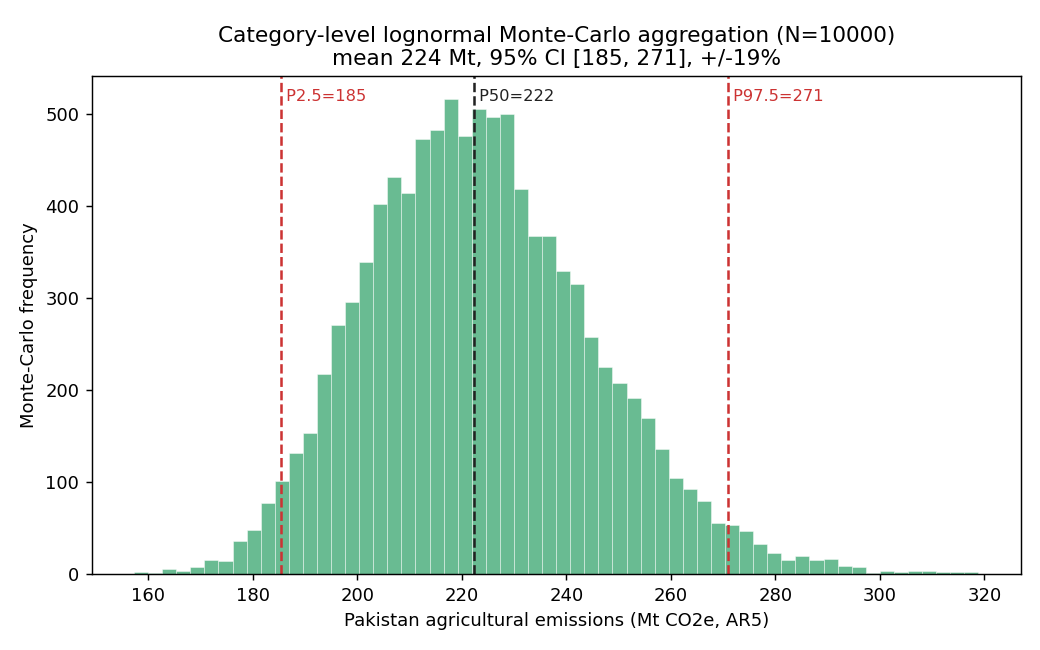
\includegraphics[width=\linewidth]{uncertainty_distribution.png}
\caption{Monte-Carlo distribution of total agricultural greenhouse-gas emissions
based on \num{10000} draws. The figure marks the median and the 2.5th and 97.5th
percentiles.}
\label{fig:uncert}
\end{figure}

\subsection{Key categories}

Four categories qualify as key under the IPCC Approach~1 level or trend assessment: enteric
fermentation, managed soils, manure management and rice cultivation. Together they account
for more than \SI{95}{\percent} of both the 2024 inventory level and the contribution to the
1990--2024 trend.

Enteric fermentation dominates the level assessment, contributing \SI{67.9}{\percent} of the
2024 total. Rice cultivation contributes only \SI{7.4}{\percent} of the 2024 level but
accounts for \SI{48.6}{\percent} of the trend assessment.

The trend result does not mean that rice emissions grew faster than the other categories.
Rice emissions increased by a factor of approximately \num{1.7} between 1990 and 2024,
compared with factors of \num{2.7}--\num{3.2} for the other major categories. Rice ranks
highly because its slower growth caused its share of the inventory to change substantially
relative to the sector average.

The four key categories include those with the widest uncertainty bands, particularly rice
cultivation and managed soils. They are therefore the highest-priority categories for
improved activity data and country-specific Tier~2 or Tier~3 emission factors.

\begin{table}[!htbp]
\centering
\footnotesize
\begin{tabular}{@{}lccc@{}}
\toprule
\textbf{Category} & \textbf{Level \%} & \textbf{Trend \%} & \textbf{Key} \\
\midrule
Enteric fermentation & 67.9 & 27.3 & \checkmark \\
Managed soils        & 12.8 &  5.0 & \checkmark \\
Manure management    &  9.5 & 17.7 & \checkmark \\
Rice cultivation     &  7.4 & 48.6 & \checkmark \\
Urea application     &  2.2 &  1.2 & \\
Field burning        &  0.3 &  0.1 & \\
\bottomrule
\end{tabular}
\caption{IPCC Approach~1 key-category assessment for agriculture. The level
assessment reports each category's share of the 2024 total. The trend assessment measures its
contribution to the change in inventory composition between 1990 and 2024. A category is
classified as key if it falls within the cumulative \SI{95}{\percent} threshold under either
assessment.}
\label{tab:keycat}
\end{table}

\subsection{Effect of correcting the livestock nitrogen boundaries}
\label{sec:results-nledger}

The shared nitrogen ledger was used to align the greenhouse-gas and air-pollutant
calculations.

Before alignment, the greenhouse-gas calculation appeared to indicate that \SI{21}{\percent}
of managed nitrogen volatilised, compared with \SI{49.5}{\percent} in the air-pollutant
calculation. This apparent difference resulted largely from comparing different stages and
chemical bases. The IPCC fractions represented both \NHthree{}-N and \NOx{}-N and separated
pre-field losses from post-application losses, whereas the EMEP/EEA calculation represented
\NHthree{}-N and followed the complete stage sequence from housing through storage and field
application.

After conversion to a common \NHthree{}-N basis, the total livestock volatilisation estimates
are relatively close. The IPCC chain gives \SI{1.967}{}~Mt \NHthree{}-N, while the EMEP/EEA
chain gives \SI{1.588}{}~Mt \NHthree{}-N. The ratio is \num{1.24}.

The stage-level comparison is less consistent. Housing and storage differ by a factor of
\num{1.25}. The IPCC field-application estimate is \num{0.65} times the EMEP/EEA value, while
the IPCC grazing estimate is \num{3.53} times the EMEP/EEA value. The similar aggregate
totals therefore result partly from offsetting stage-level differences.

The greenhouse-gas inventory retains the IPCC nitrogen-accounting chain because the inventory
is reported under IPCC methods. The air-pollutant calculation retains the EMEP/EEA
stage-resolved method because ammonia losses must be assigned to housing, storage, grazing
and field application. Replacing the IPCC loss formulation with the EMEP/EEA formulation in
the greenhouse-gas pathway would change the national total by only approximately
\SI{0.24}{}~Mt~\COe{}. The choice of representation is therefore based mainly on
methodological scope rather than on its effect on the headline total.

Correcting the earlier IPCC nitrogen chain reduced the quantity of manure nitrogen reaching
soils from \SI{2.72}{} to \SI{2.33}{}~Mt~N. This lowered the agricultural greenhouse-gas
total by \SI{0.62}{}~Mt~\COe{}, from \SI{221.71}{} to \SI{221.09}{}~Mt~\COe{}. A subsequent
update to the synthetic-fertiliser factor produced \SI{221.2}{}~Mt~\COe{}; the
harmonisation round's activity refresh and the rc39 herd re-base then carried the published
total to \SI{223.5}{}~Mt~\COe{}. Supplementary Note~S5 documents the corrections.

The correction does not change livestock \NHthree{}, because the air-pollutant module reads
the managed and grazing nitrogen pools directly rather than deriving ammonia from the final
manure-applied pool.

The common ledger guarantees that the same nitrogen is not assigned to multiple stages or
omitted between them. It does not require the IPCC and EMEP/EEA methods to produce identical
volatilised masses within each stage.

\begin{table}[!htbp]
\centering
\footnotesize
\begin{tabular}{@{}lrr@{}}
\toprule
\textbf{Flow} & \textbf{Mt N} & \textbf{\% excreted} \\
\midrule
\multicolumn{3}{@{}l}{\emph{A. Excretion partition}} \\
Total N excreted                          & 7.78 & 100.0 \\
\quad to grazing ($F_{PRP}$)                & 3.18 & 40.9 \\
\quad to managed systems                  & 3.34 & 42.9 \\
\quad diverted as dung-cake fuel (to Energy) & 1.26 & 16.2 \\
\midrule
\multicolumn{3}{@{}l}{\emph{B. Pre-field management (Eq.~10.34a)}} \\
\NHthree{}-N + \NOx{}-N ($\mathrm{Frac_{GasMS}}$) & 0.91 & 11.7 \\
leaching, N\textsubscript{2}, and \NtwoO{}-N          & 0.09 &  1.2 \\
\quad = N available for application ($F_{ON}$) & 2.33 & 30.0 \\
\midrule
\multicolumn{3}{@{}l}{\emph{C. Field application, gross basis (Ch.~11)}} \\
direct soil \NtwoO{}-N ($EF_1$)           & 0.01 &  0.1 \\
\NHthree{}-N + \NOx{}-N ($\mathrm{Frac_{GASM}}$) & 0.49 &  6.3 \\
leaching/run-off                          & 0.45 &  5.8 \\
\quad = retained in the soil nitrogen pool & 1.38 & 17.8 \\
\midrule
\multicolumn{3}{@{}l}{\emph{Same managed pool on the EMEP/EEA TAN basis}} \\
housing, yards and storage \NHthree{}-N   & 0.69 &  8.9 \\
field-application \NHthree{}-N            & 0.71 &  9.2 \\
\bottomrule
\end{tabular}
\caption{National livestock nitrogen ledger for 2024. The IPCC chain tracks
excreted nitrogen through grazing, managed systems, pre-field losses, field application,
leaching and retention in soils. The EMEP/EEA rows provide a parallel TAN-based representation
of ammonia losses from the same managed nitrogen pool.
Generated by
\texttt{src/pkinv/sectors/agriculture/n\_ledger.py}.}
\label{tab:nledger}
\end{table}

\begin{table}[!htbp]
\centering
\footnotesize
\begin{tabular}{@{}lrrr@{}}
\toprule
\textbf{Stage} & \textbf{IPCC} & \textbf{EMEP} & \textbf{Ratio} \\
\midrule
Housing + storage   & 0.866 & 0.694 & 1.25 \\
Field application   & 0.466 & 0.714 & \textbf{0.65} \\
Grazing             & 0.635 & 0.180 & \textbf{3.53} \\
\midrule
\textbf{Total}      & \textbf{1.967} & \textbf{1.588} & \textbf{1.24} \\
\bottomrule
\end{tabular}
\caption{Livestock ammonia losses by stage after conversion to a common
\NHthree{}-N basis. The IPCC and EMEP/EEA totals are similar, but field-application and grazing
estimates differ substantially in opposite directions.
Generated by \texttt{src/pkinv/sectors/agriculture/n\_ledger.py}.}
\label{tab:stages}
\end{table}
